\documentclass[tikz,border=8pt]{standalone}
\usepackage{tikz}
\usepackage{amsmath}
\usepackage{helvet}
\renewcommand{\familydefault}{\sfdefault}
\usetikzlibrary{positioning,arrows.meta,fit,backgrounds,calc,decorations.pathreplacing}

\begin{document}
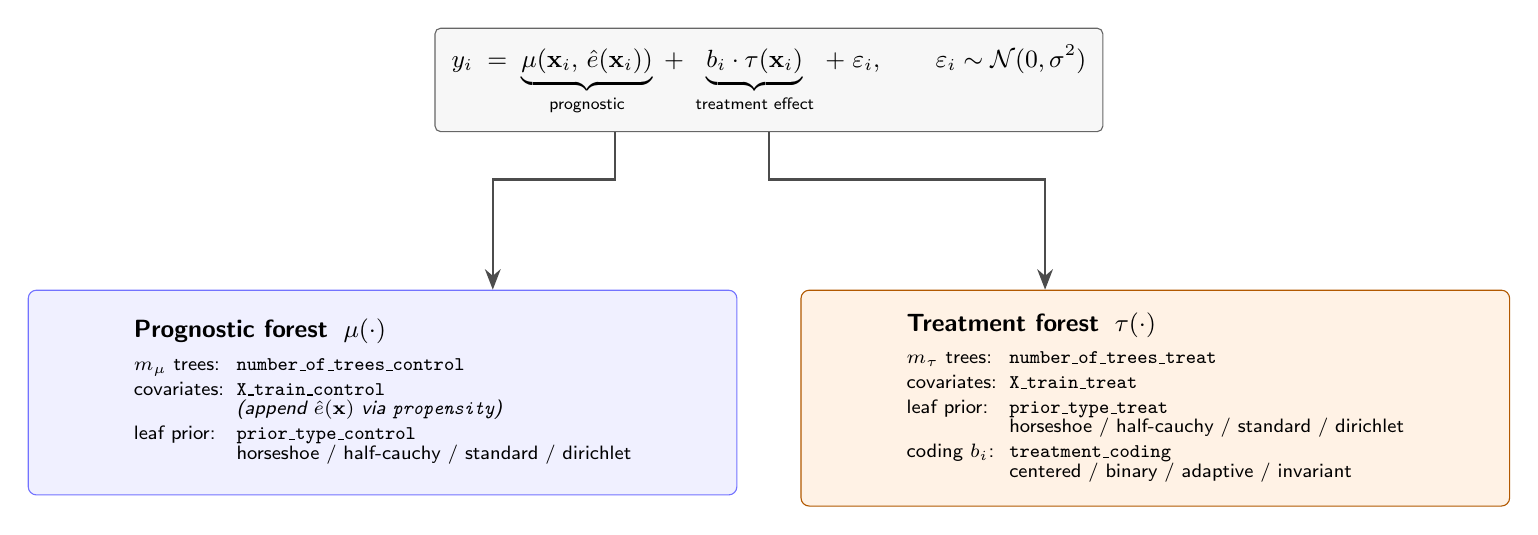
\begin{tikzpicture}[
  font=\small,
  >={Stealth[length=2.6mm,width=2.0mm]},
  eqbox/.style={
    draw=black!60, rounded corners=2pt, align=center,
    inner sep=6pt, minimum height=10mm, fill=black!3
  },
  forest/.style={
    draw=black!70, rounded corners=3pt, align=left,
    inner sep=8pt, minimum height=26mm, minimum width=90mm,
    fill=white
  },
  mubox/.style={forest, fill=blue!6,   draw=blue!55},
  taubox/.style={forest, fill=orange!10, draw=orange!70!black},
  arrow/.style={->, thick, black!70},
  note/.style={font=\scriptsize\itshape, black!60}
]

% ---------- Row 1: model equation ----------
\node[eqbox] (eq) {$\displaystyle
  y_i \;=\; \underbrace{\mu(\mathbf{x}_i,\, \hat e(\mathbf{x}_i))}_{\text{prognostic}}
           \;+\; \underbrace{b_i \cdot \tau(\mathbf{x}_i)}_{\text{treatment effect}}
           \;+\; \varepsilon_i,
  \qquad \varepsilon_i \sim \mathcal{N}(0, \sigma^2)$};

% ---------- Row 2: the two forests ----------
\node[mubox,  below left=20mm and 4mm of eq.south]  (mu) {
  \textbf{Prognostic forest} $\;\mu(\cdot)$\\[3pt]
  \scriptsize
  \begin{tabular}{@{}l@{\hspace{0.6em}}l@{}}
    $m_\mu$ trees:  & \texttt{number\_of\_trees\_control}\\[1pt]
    covariates:     & \texttt{X\_train\_control}\\[-1pt]
                    & \textit{(append $\hat e(\mathbf{x})$ via \texttt{propensity})}\\[1pt]
    leaf prior:     & \texttt{prior\_type\_control}\\[-1pt]
                    & horseshoe / half-cauchy / standard / dirichlet\\
  \end{tabular}
};

\node[taubox, below right=20mm and 4mm of eq.south] (tau) {
  \textbf{Treatment forest} $\;\tau(\cdot)$\\[3pt]
  \scriptsize
  \begin{tabular}{@{}l@{\hspace{0.6em}}l@{}}
    $m_\tau$ trees: & \texttt{number\_of\_trees\_treat}\\[1pt]
    covariates:     & \texttt{X\_train\_treat}\\[1pt]
    leaf prior:     & \texttt{prior\_type\_treat}\\[-1pt]
                    & horseshoe / half-cauchy / standard / dirichlet\\[1pt]
    coding $b_i$:   & \texttt{treatment\_coding}\\[-1pt]
                    & centered / binary / adaptive / invariant\\
  \end{tabular}
};

% Two separate arrows from the corresponding parts of the equation to each
% forest. Origins are placed under the prognostic and treatment-effect
% subexpressions via fractional positions along the eq.south edge.
\draw[arrow] ($(eq.south west)!0.27!(eq.south east)$) -- ++(0,-6mm) -| ($(mu.north)+(14mm,0)$);
\draw[arrow] ($(eq.south west)!0.50!(eq.south east)$) -- ++(0,-6mm) -| ($(tau.north)-(14mm,0)$);

\end{tikzpicture}
\end{document}
